\documentclass[aspectratio=169]{beamer}
\usepackage{color,amsmath}
\usepackage{subfigure}
\usepackage{booktabs}
\usepackage{framed}
\usepackage{comment}

\def\vf{\vfill}

%%%%%%%%%%%%%%%%%%%%%%%%%%
\title[]{Moving beyond simple experiments\\(04-04)}
\author[]{Matthew J. Salganik\\Department of Sociology\\Princeton University}
\date[]{Soc 596: Computational Social Science\\Fall 2016
\vfill
\begin{flushright}
\vspace{0.6in}

\includegraphics[width=0.1\textwidth]{figures/cc.png}
\end{flushright}
}
\begin{document}
%%%%%%%%%%%%%%%%%%%%%%%%%%
\frame{\titlepage}
%%%%%%%%%%%%%%%%%%%%%%%%%%
\begin{frame}

\Large{
\begin{center}
Optimization experiments vs  Understanding experiments
\end{center}
}

\end{frame}
%%%%%%%%%%%%%%%%%%%%%%%
\begin{frame}

\Large{
\begin{center}
Optimization experiments + Understanding experiments
\end{center}
}

\end{frame}
%%%%%%%%%%%%%%%%%%%%%%%
\begin{frame}

\begin{figure}
  \centering
  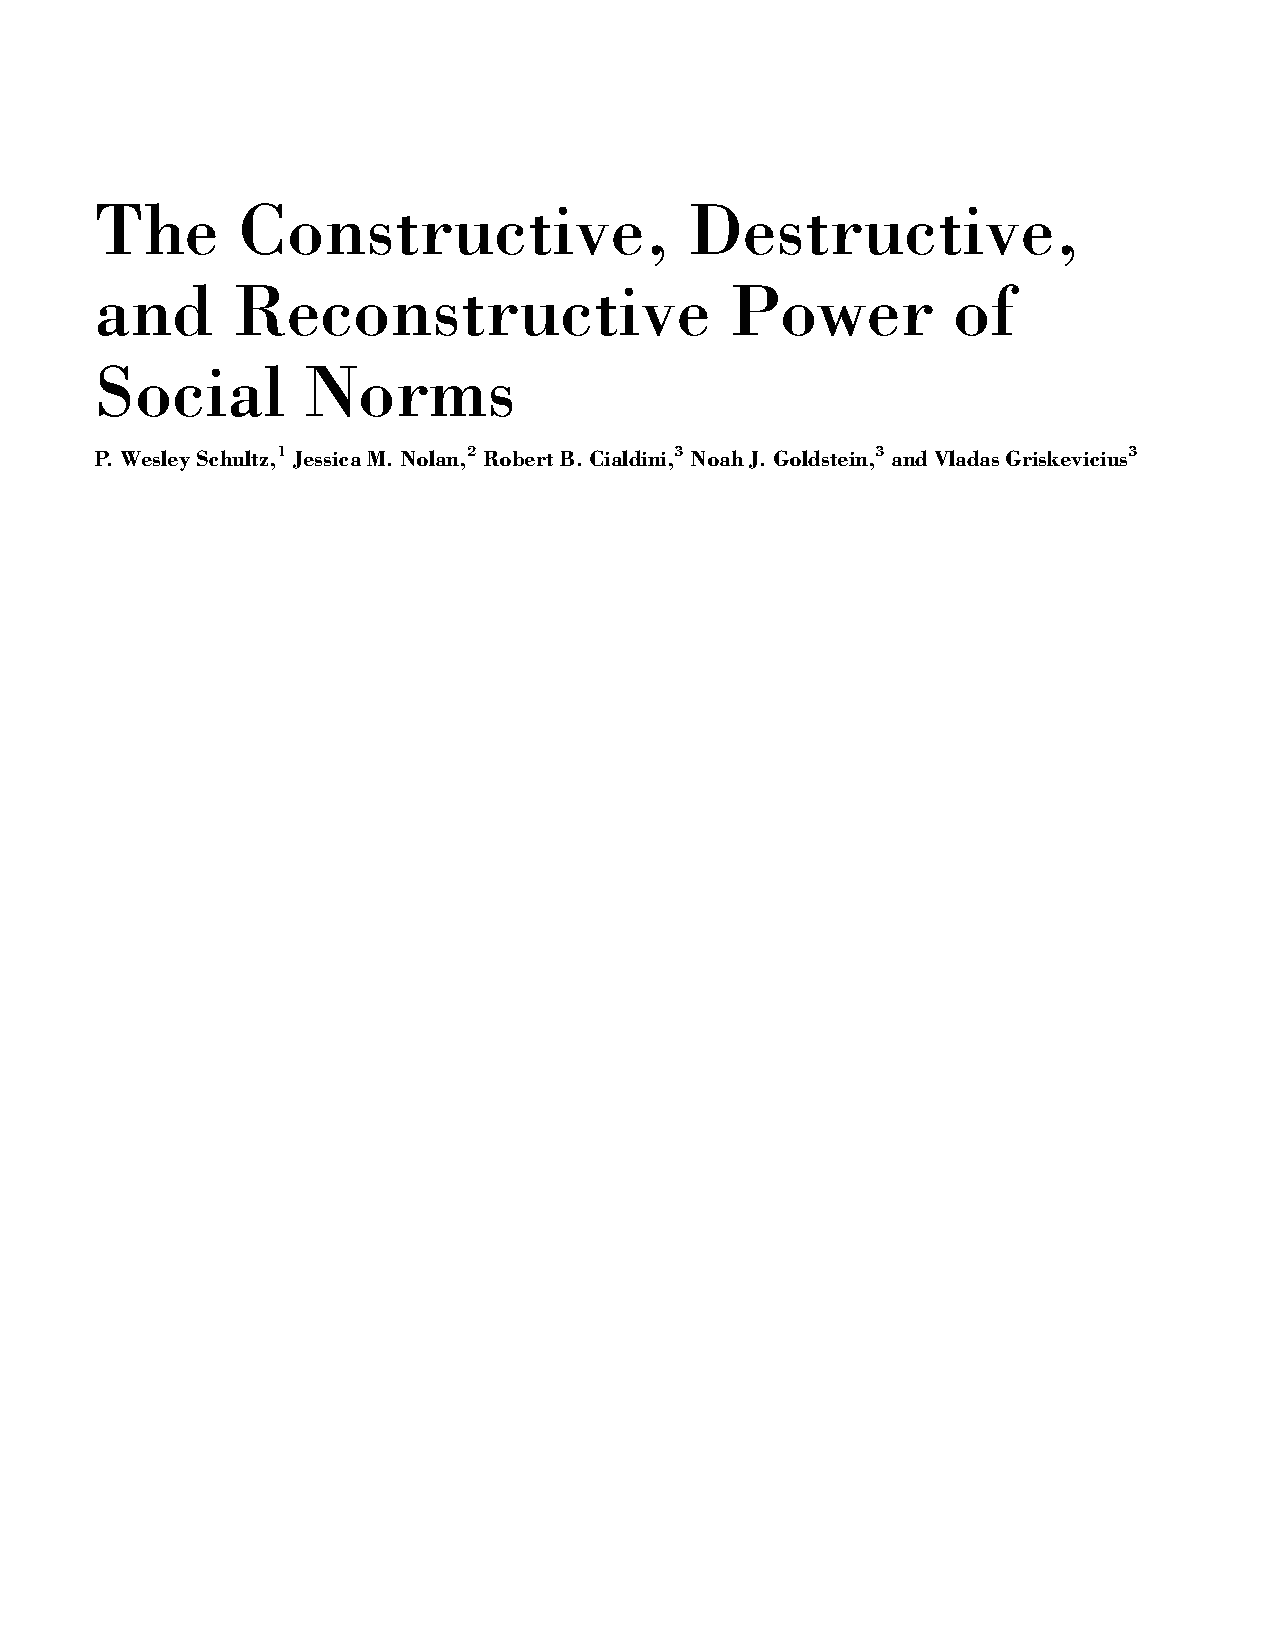
\includegraphics[width = 0.9\textwidth]{figures/schultz_constructive_2007_title}
\end{figure}

\vf
\tiny{\url{http://dx.doi.org/10.1111/j.1467-9280.2007.01917.x}}

\end{frame}
%%%%%%%%%%%%%%%%%%%%%%%
\begin{frame}

\begin{figure}
  \centering
  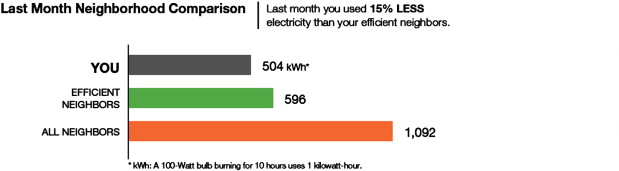
\includegraphics[width = \textwidth]{figures/energy_peers_no_emoticon}
\end{figure}

\vf
\tiny{Figures from Allcott (2011)}

\end{frame}
%%%%%%%%%%%%%%%%%%%%%%%%
\begin{frame}

\begin{figure}
  \centering
  \only<1>{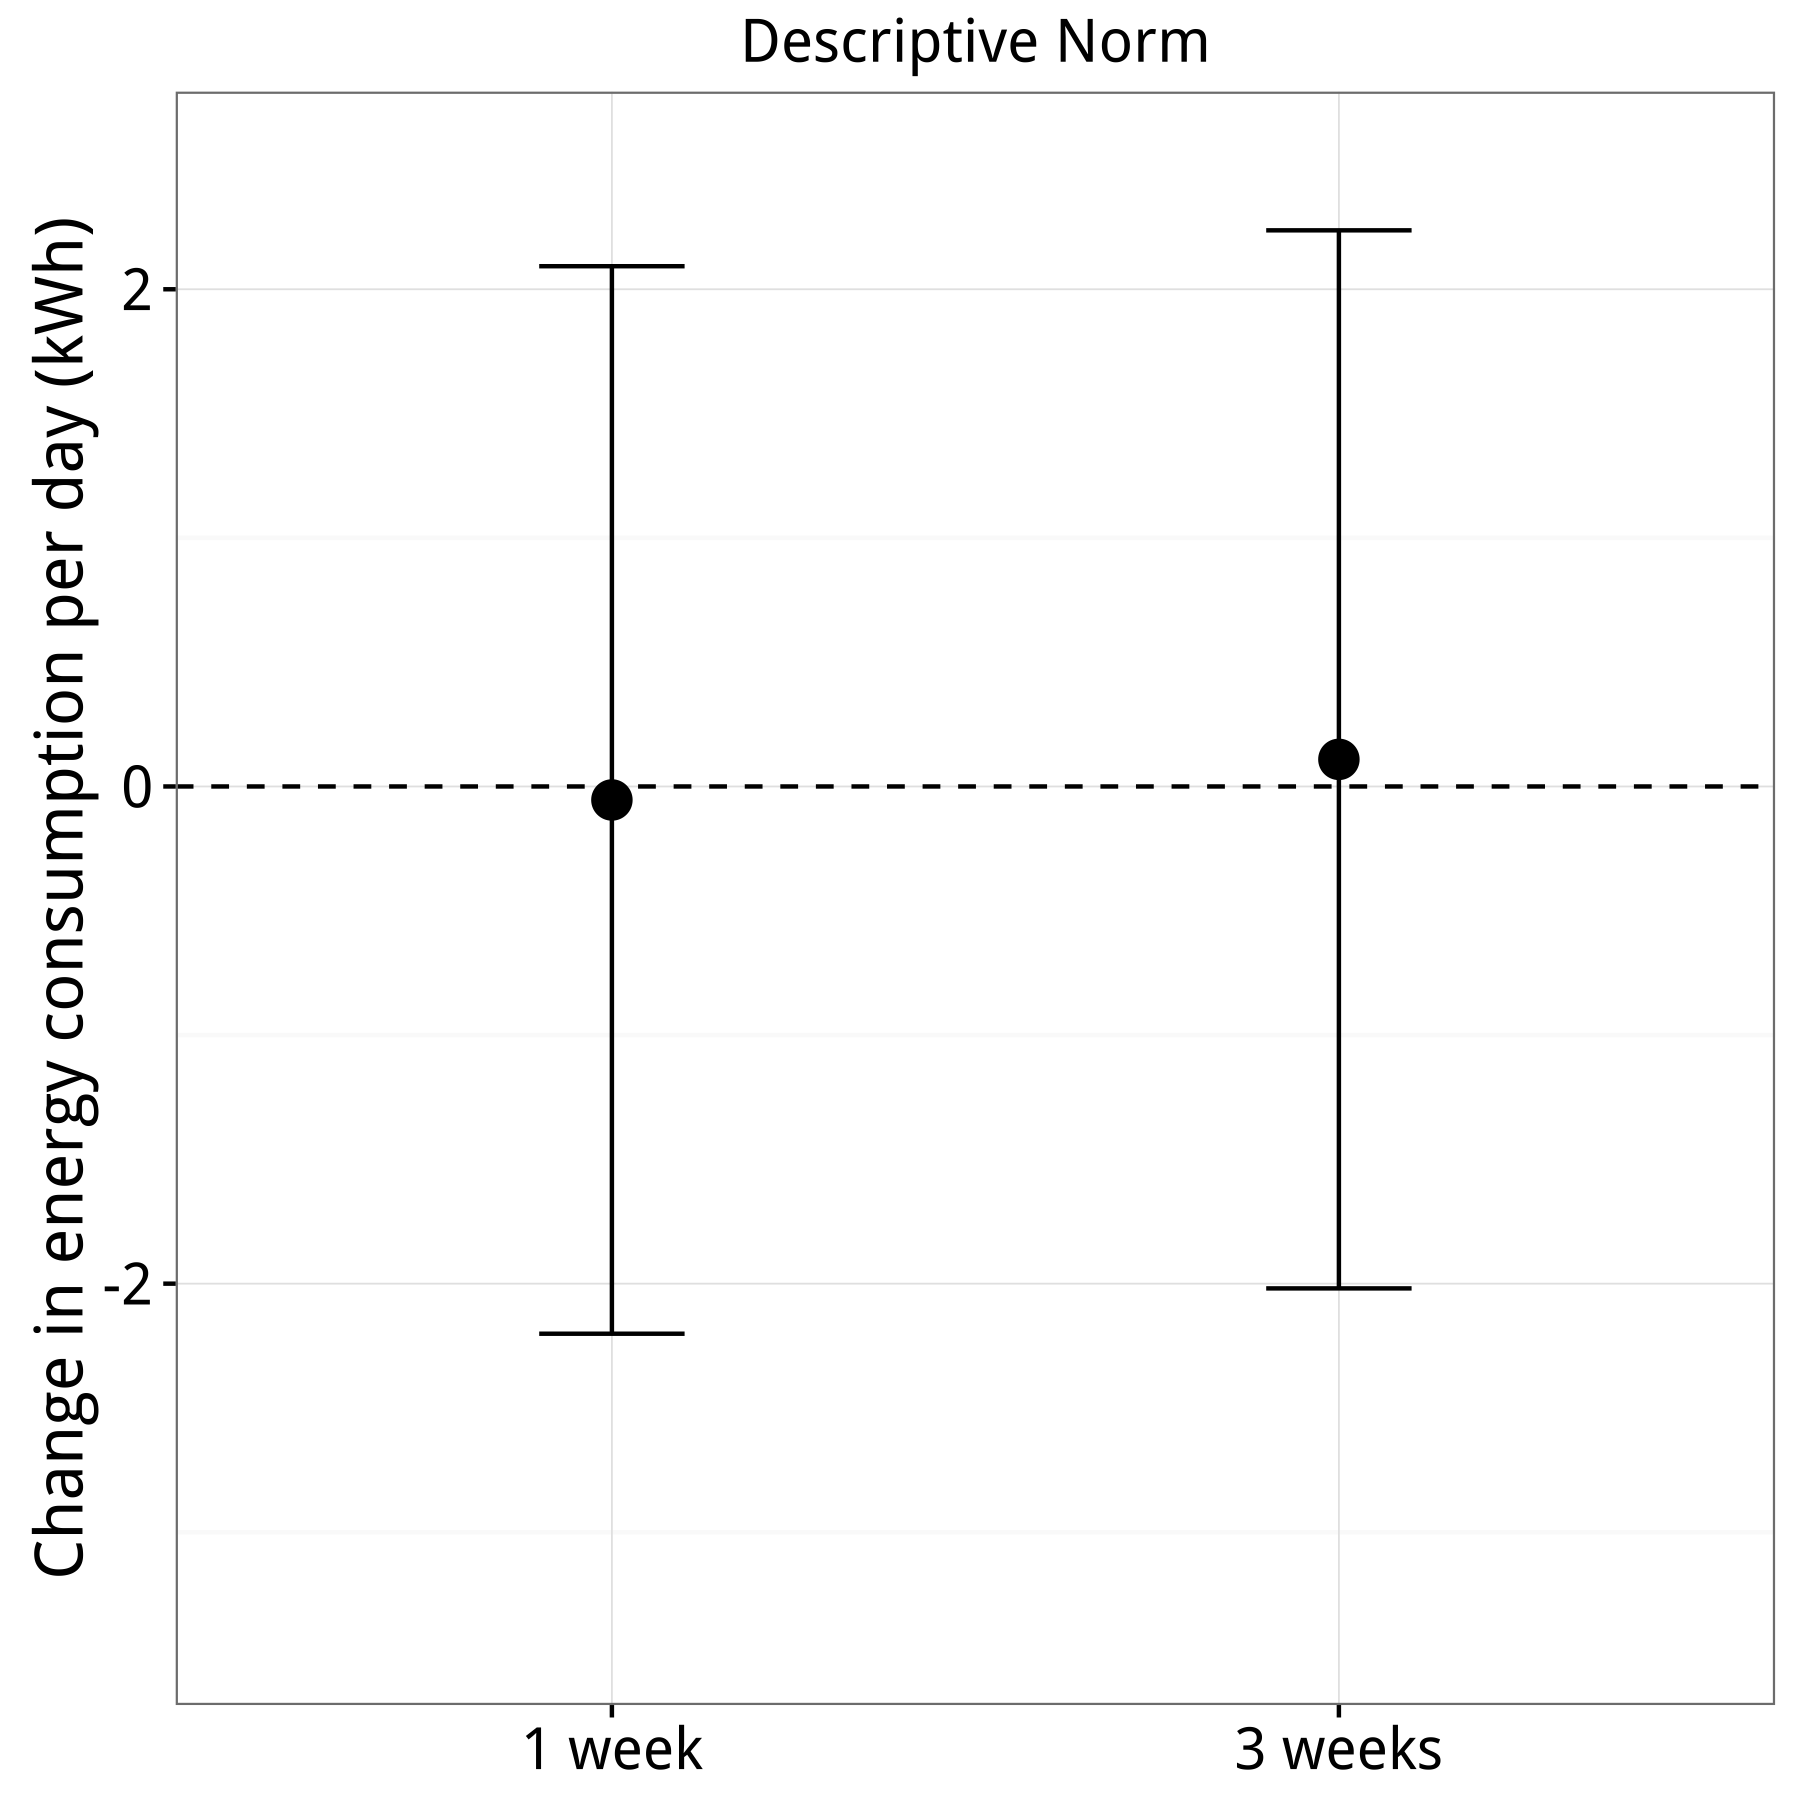
\includegraphics[width = 0.5\textwidth]{figures/schultz_constructive_2007_1panel}}
  \only<2>{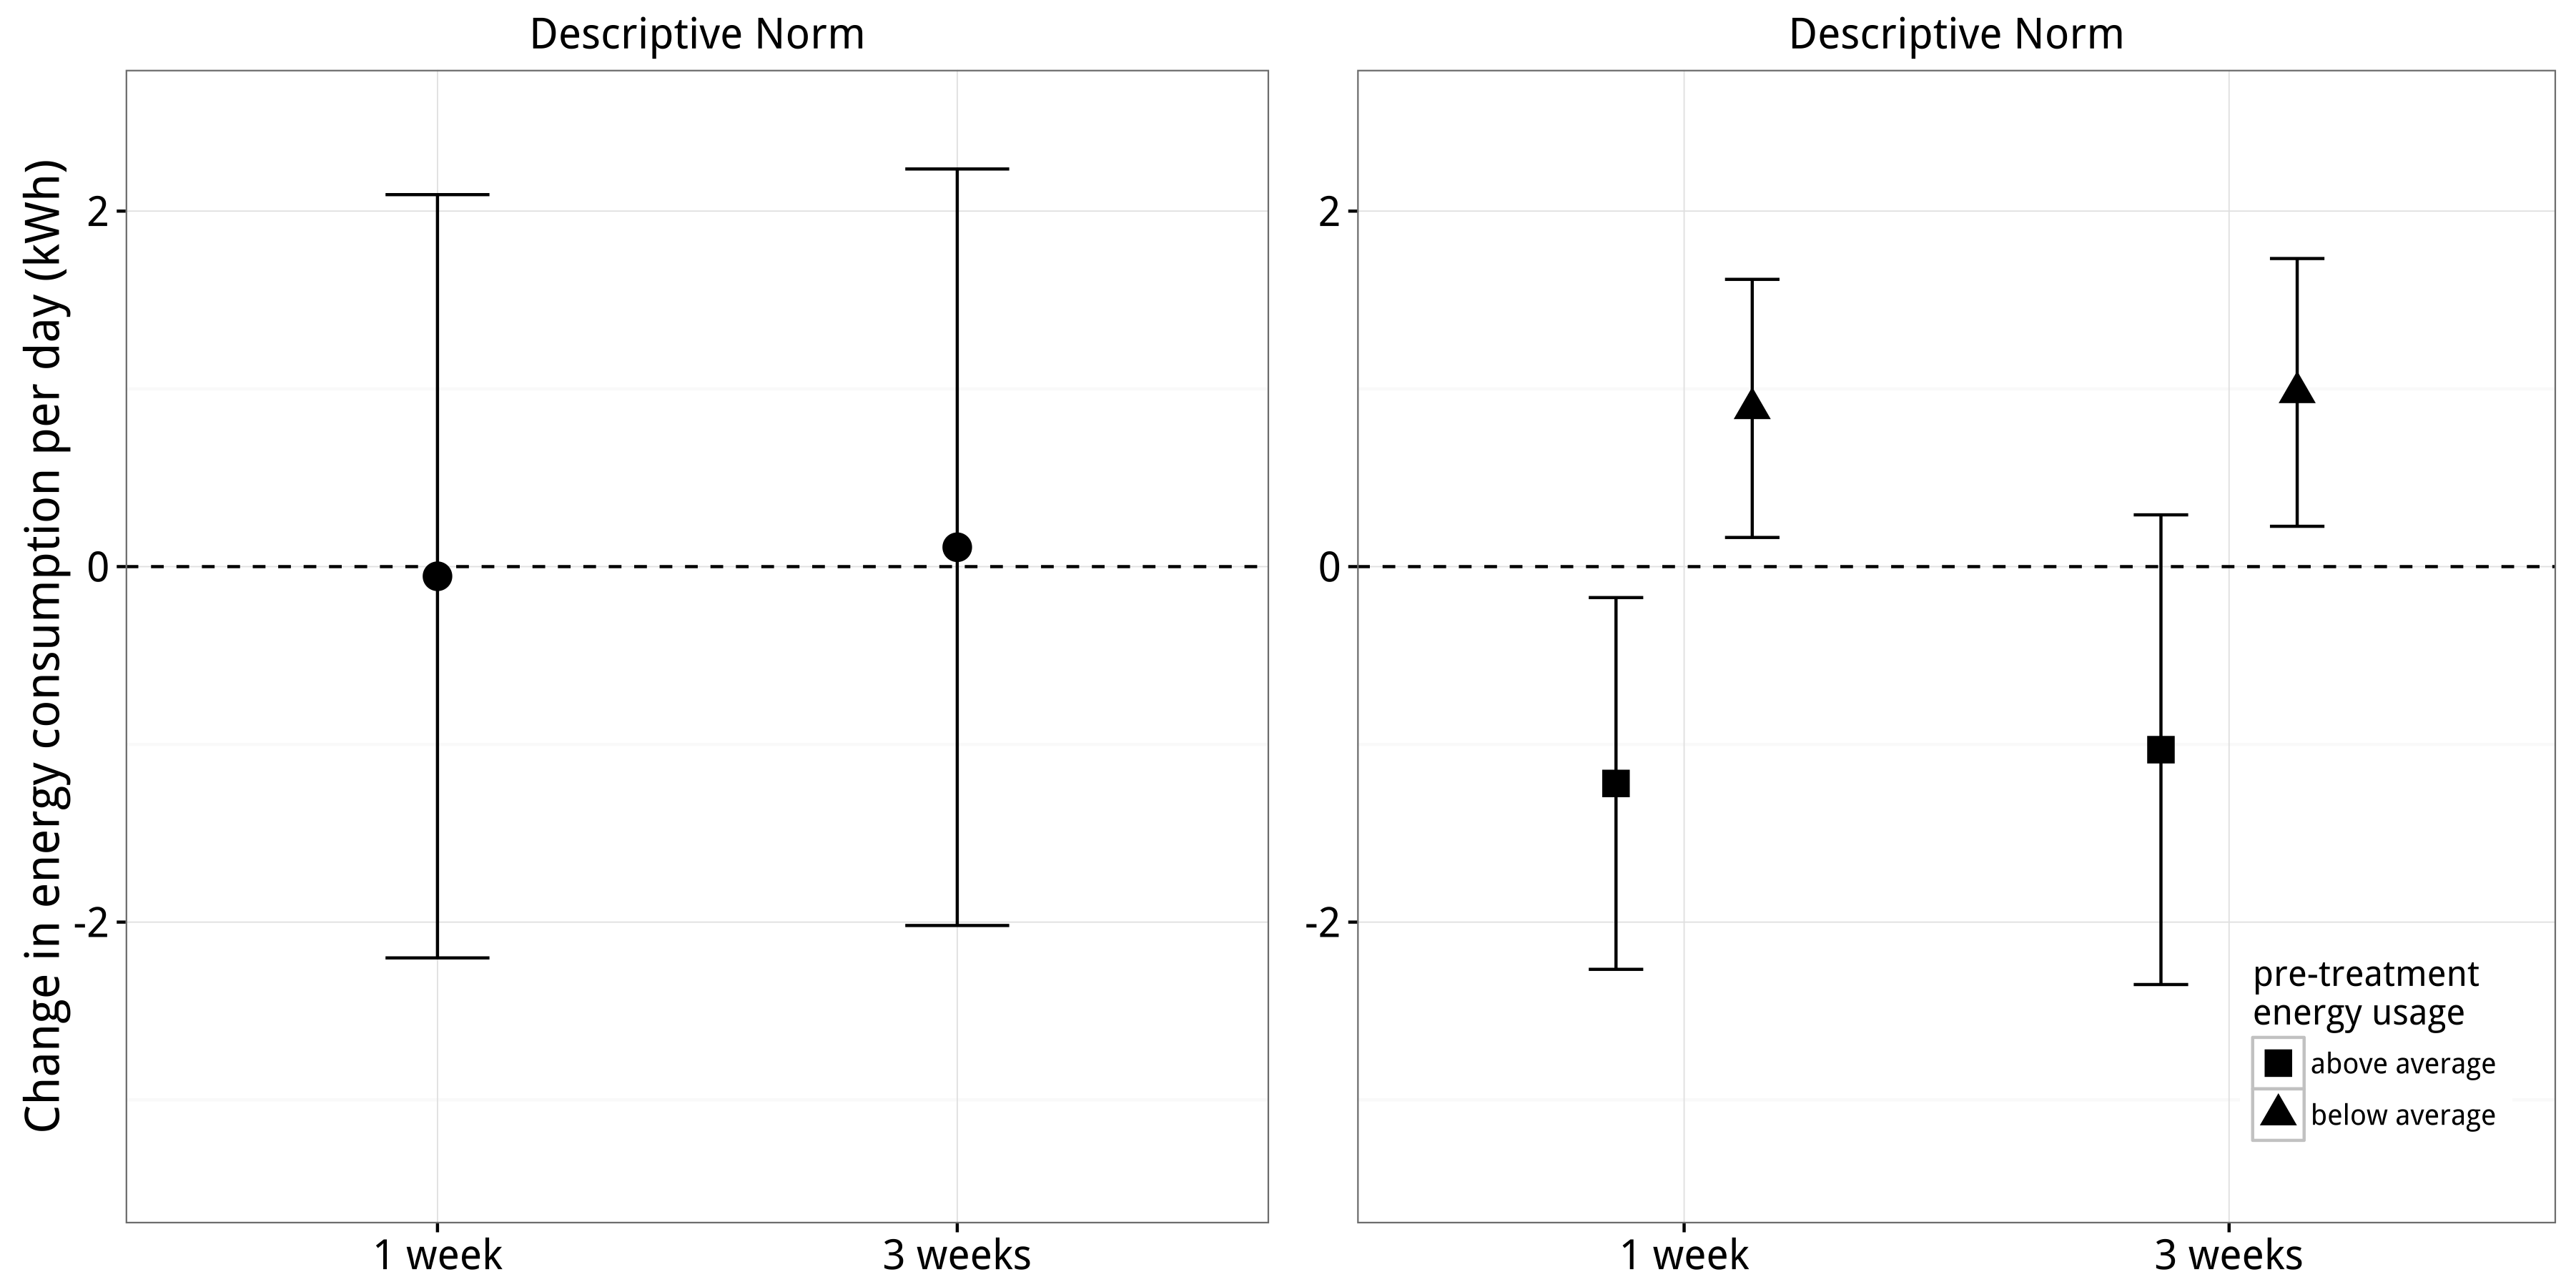
\includegraphics[width = 0.8\textwidth]{figures/schultz_constructive_2007_2panel}}
\end{figure}

\end{frame}
%%%%%%%%%%%%%%%%%%%%%%%%
\begin{frame}

\begin{figure}
  \centering
  \only<1>{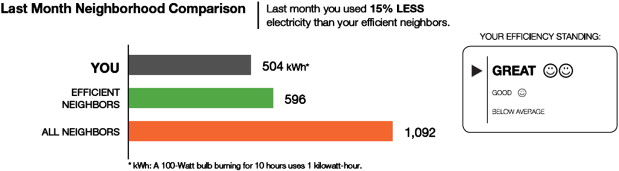
\includegraphics[width = \textwidth]{figures/allcott_social_2011_fig1}}
  \only<2>{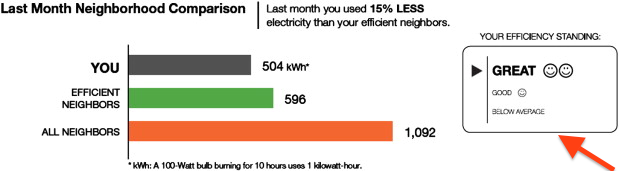
\includegraphics[width = \textwidth]{figures/allcott_social_2011_fig1_arrow}}
\end{figure}

\vf
\tiny{Figures from Allcott (2011)}

\end{frame}
%%%%%%%%%%%%%%%%%%%%%%%%
\begin{frame}

\begin{figure}
  \centering
  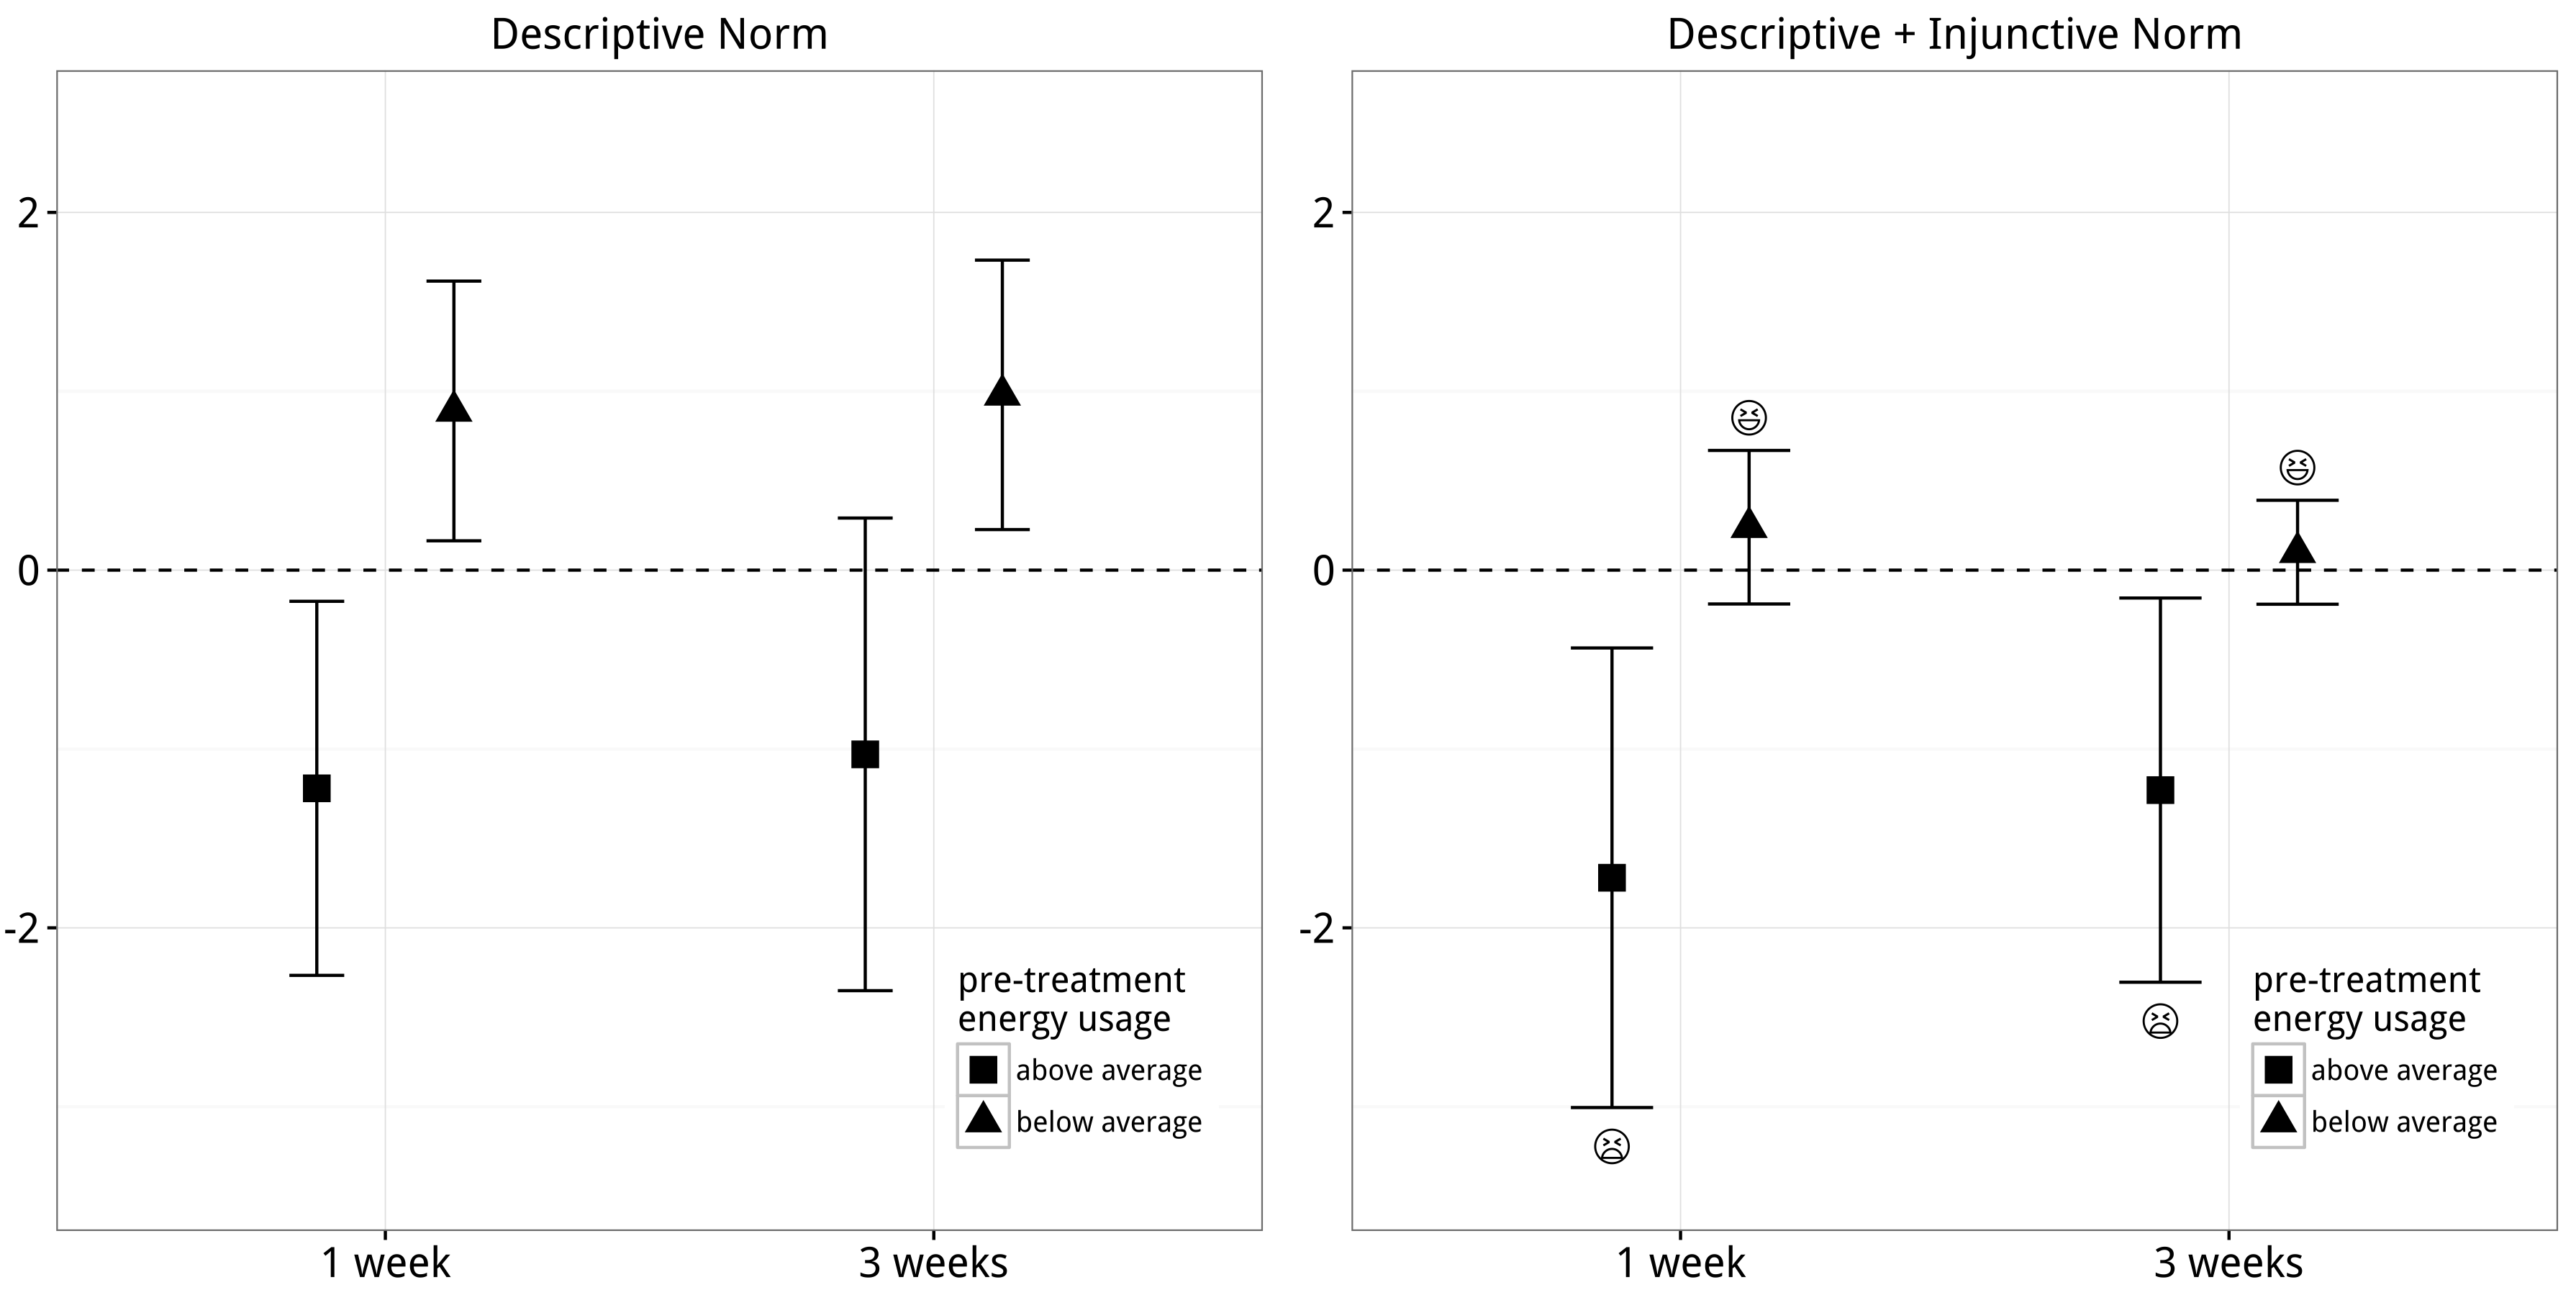
\includegraphics[width = \textwidth]{figures/schultz_constructive_2007_23panel}
\end{figure}

\end{frame}
%%%%%%%%%%%%%%%%%%%%%%%%
\begin{frame}

If you want to move beyond simple experiments:
\begin{itemize}
\item Heterogeneity of treatment effects
\item External validity
\item Mechanisms
\end{itemize}

\end{frame}
%%%%%%%%%%%%%%%%%%%%%%%%%%%


\end{document}
